\section{Концентрирующая решетка}

С концентрирующей решеткой ситуция похожая, можем заметить что гибающая это 
\begin{equation}
    \inner{\cfrac{\sin \inner{\cfrac{kd}{2}\cos{\gamma} 
    \inner{\sin \inner{x - \gamma} - \sin{\gamma}}}}
    {\cfrac{kd}{2}\cos{\gamma} 
    \inner{\sin \inner{x - \gamma} - \sin{\gamma}}}}^2 .
\end{equation}
Эта функция похожа на ту что была для пропускающей решотки но теперь 
максимум огибающей сдвинут относительно центра. Выведу данные на график:
\begin{figure}[h]
    \centering
    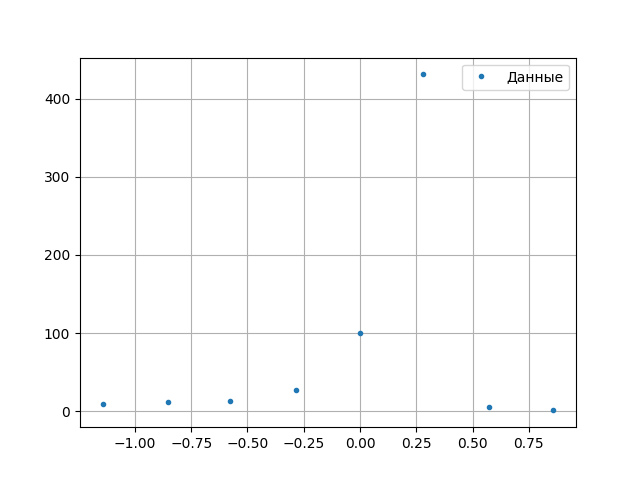
\includegraphics[trim={0 0 0 0},clip,width=\textwidth]{Ex_3/ex_2_dat.png}
    \caption{}
    \label{Ex_2_2}
\end{figure}
Заметим что огибающая дает наибольший влад в 0, 1 максимумы. Но всетики 1 максимум 
значительно больше значит уже сейчас можно оценить $\gamma$:
\begin{equation}
    \sin(x - \gamma) - \sin \gamma = 0 \implies x = 2\gamma
\end{equation}
$\gamma \approx 0.14$.d можно нати также как и в предыдущем эксперементе, 
$d \approx 2.45\cdot 10^{-6}m$.

теперь юолее точно подберем $\gamma$, получим $\gamma \approx 0.09$ 
\begin{figure}[h]
    \centering
    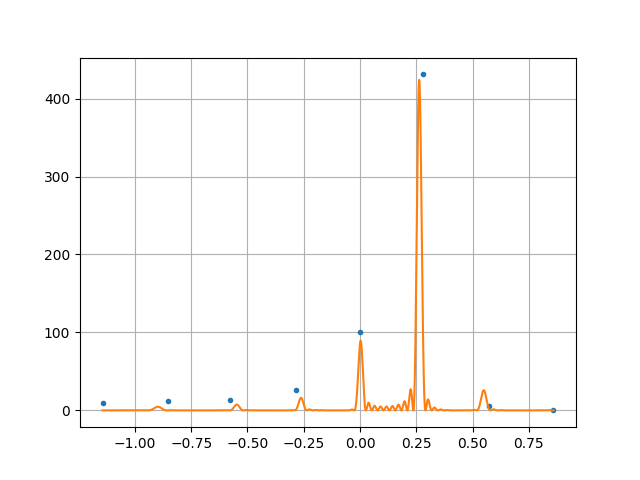
\includegraphics[trim={0 0 0 0},clip,width=\textwidth]{Ex_3/ex_2_approx.png}
    \caption{}
    \label{Ex_2_3}
\end{figure}

